%*******************************************************************************
%*********************************** First Chapter *****************************
%*******************************************************************************

\chapter{Introduction}  %Title of the First Chapter
\label{cha:intro}

\ifpdf
    \graphicspath{{Chapter1/Figs/Raster/}{Chapter1/Figs/PDF/}{Chapter1/Figs/}}
\else
    \graphicspath{{Chapter1/Figs/Vector/}{Chapter1/Figs/}}
\fi

% **************************** Chapter Abstract ******************************
\leftskip=1cm
\noindent
\emph{This introductory chapter provides the motivation of the thesis, enumerates the examined questions, and outlines the adopted approach to answer them. Additionally, the organization, position, and scope of the thesis are presented.}

\leftskip=0pt\rightskip=0pt

%******************************************************************************************
%******************************************************************************************
\section{Motivation} % GENERAL
% !!CEN document from Mirek, importance of the topic is highlighted!!

Probabilistic models in engineering are generally underappreciated and underdeveloped compared with physical ones. However, this unbalanced attention is not justified by their lower importance, since the same relative improvement in probabilistic models might yield to greater savings than that in physical models. \mynote{(\ref{}), figure showing a small example} In other words, advances in physical models are typically outweighed by the uncertainties in the probabilistic ones \citep{Mcrobie2004}. This study aspires to subtly adjust this imbalance by focusing on probabilistic models through investigating the effect of conventional engineering simplifications in structural reliability. Due to the vast range and diversity of probabilistic analysis, a sharp focus is needed for efficacy, thus this study is restricted to probabilistic models of extreme\footnote{Hereinafter extremes refers to structural engineering extremes, values that govern the design of load bearing structures. Their return period can vary from 50 to 10000 years.} ground snow loads. Despite the restricted subject\mynote{scope}, many of the considered issues are the same for other basic variables, especially climatic actions; hence, it is hoped that the findings presented here will be utilized for those as well.

\mynote{
A possible interpretation of engineering is as an activity of making abstract models, analyzing, and finally realizing them (Figure \ref{fig:mod_overview}). The model is composed of two main components: physical and probabilistic models. Both are indispensable
to reliably fulfill the needs which spurred the engineering activity. The former comprises for example the mechanical models of resistances while the latter represents our incomplete state of knowledge and uncertainty of the involved variables, these are commonly described with distribution functions and random processes.
Structural design standards, e.g. Eurocode, AISC, AASHTO, are invariably focused on physical models and the probabilistic component is relatively underdeveloped/rudimentary. Nowadays, most of the research effort is still devoted to the improvement of the physical models; however, this disproportional development renders its advances less effective, e.g. the impact of 10\% improvement in a resistance model of structural members is outweighed by the uncertainties in the probabilistic load models. Therefore, it appears that civil engineering can be more efficiently advanced by focusing on the probabilistic models.

\begin{figure}[htbp!]
	\centering    
	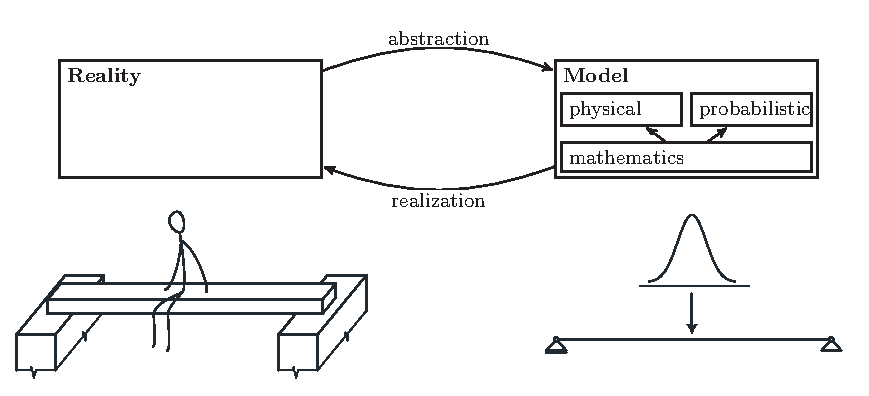
\includegraphics[width=0.8\textwidth]{modeling_overview_all.pdf}
	\caption{Concept of modeling with its main components.}
	\label{fig:mod_overview}
\end{figure}
}   


%******************************************************************************************
%******************************************************************************************
\section{Problem statement} % SPECIFIC
\label{sec:prob_state}

Snow is an important climatic action, which governs the reliability of many structures, particularly of lightweight roofs. These should operate without major structural maintenance for typically 50 years, and their real working life often spans over 100 years. Therefore, it is of utmost importance that the expected actions are adequately anticipated during the design process.

The topic selection is partially motivated by the relatively large number of structural damages and collapses experienced around the world due to snow loads \citep{Geis2011}; e.g. recently in 2005/06 Central Europe, 2010/11 North-Eastern USA. One of the diverse causes of collapses appears to be the inadequate safety level provided by standards \citep{Holicky2009, Meloysund2010}. Further motivations for the study are the perceived inconsistencies in the current European standard regarding exceptional ground snow load, and statistical treatment of snow measurements. The problems seem to be urgent particularly for lowland areas with continental climate where exceptional snowfalls are more likely than in mountains \citep{Sanpaolesi1998}. Thus, the topic has a great importance for Hungary and for neighboring countries. The relevance of the topic is also highlighted by a foreseen revision of design procedures within Eurocode. 

The main issues examined in this study -- with brief description and related questions -- are summarized below:

\begin{enumerate}
	\item There is a lack of agreement among reliability experts on the appropriate distribution function for ground snow maxima. Critical examination of current probabilistic snow models and application of statistically established methods are needed. \textit{Which distribution function is the ``best'' to model ground snow extremes? What constitutes an appropriate model?}
	
	\item Statistical uncertainties -- arising from scarcity of observations -- are typically neglected; however, they seem to be important as observation periods are only a small fraction of governing return periods, thus extrapolation to unobserved ranges is inevitable. \textit{How large is the effect of statistical uncertainties on structural reliability? Is their neglect reasonable? How should these uncertainties be taken into account?}
	
	\item Measurements are inevitably contaminated with measurement uncertainty, which is especially important for snow where measuring techniques are often burdened with large uncertainty. \textit{How measurement uncertainty should be taken into account and propagated to structural reliability? Is the current practice, which neglects it, acceptable from reliability point of view? Is its effect on failure probability practically significant?}
	
	\item Current civil engineering provisions are based on the assumption of stationarity; however, recent observations and climate models challenge this. \textit{Is the stationary assumption tenable for snow extremes? What are the practical implications of time-trends for structural reliability?}
	
	%\item Exceptional ground snow load is a ``new action'' in Eurocode that is governing the design of many lightweight structures. Yet, no definition is given in the standard and there is a confusion whether to consider it.  \textit{Is exceptional ground snow load justified from meteorological, statistical, or reliability point of view? What can be a rational definition of it? How large its value should be?}
	
	\item Correlation structure of stochastic processes is almost solely described by Gauss copula; however, this assumption is not corroborated by empirical evidence. \textit{How large is the effect of copula assumption on time-variant structural reliability? Is the current practice conservative for snow loads? How can the copula function uncertainty be treated?}		
\end{enumerate}

%All of these questions are practically motivated and investigated with bearing in mind 

\mynote{
The dominant components, sources of uncertainty are actions, their accurate modeling is important.
Comparative study between Poland and South Africa: Wind climates, the related damage and implications of adopting the Eurocode for wind action on buildings Section 4.1
motivation for wind loads
}


%******************************************************************************************
%******************************************************************************************
\section{Adopted approach}
\label{sec:solu_strat}

To explore the questions listed in Section \ref{sec:prob_state}, methods of structural reliability, mathematical statistics, and conventional civil engineering are applied. The general rationale of the investigations is the same: 
\begin{enumerate}
	\item Identification of potential gaps in current body of knowledge and/or non-conservative assumptions in practice.
	\item Examination of the underlying concepts to support hypothesis formulation, then selection or development of tools for quantitative analysis of the identified questions. 
	\item Qualitative and quantitative comparison of popular civil engineering approaches with more advanced statistical techniques that are able to capture in the former neglected effects.
	\item Parametric analysis using minimal\footnote{Minimal is used in the sense of minimal working example of programming. As simple as possible to capture the essential features of examined issue, but not simpler.} reliability problems that represent generic structures. Consideration of an extended parameter range to cover random variables other than ground snow intensity too.
	\item Illustration of the effects and proposed approaches with real-life examples.
	\item Discussion of the question and results from a broader, decision making perspective.
	\item Formulation of practical recommendations and simplified rules.
\end{enumerate}

\mynote{The latter serve as reference points as they are more sophisticated than those prevalently used in structural reliability and for calibration of standards.}

%******************************************************************************************
%******************************************************************************************
\section{Structure of the thesis}
\label{sec:organization}

The thesis' organization is presented in Figure \ref{fig:thesis_overview}.
After the introduction, an overview of the applied methods and terminology is presented (Chapter \ref{cha:overview}). Then each subsequent chapters (\ref{cha:stat_unc}-\ref{cha:copula}) deal with one or two research questions. These are similarly structured and accompanied with application examples that are intended to highlight the practical importance of the questions and feasibility of proposed approaches. These question-chapters are loosely connected and these connections are indicated by dashed lines in Figure \ref{fig:thesis_overview}. Finally, the study concludes with the summary of the contributions (Chapter \ref{cha:summary}). The appendices gather supplementary materials and technical details in an extent to allow reproducibility. Further supporting materials are available from the following GitHub account: \url{https://github.com/rozsasarpi}.

\begin{figure}[htbp!] 
	\centering
	\begin{tikzpicture}[->,>=stealth',shorten >=1pt,auto,
		thick,main node/.style={circle,draw,
		font=\large\bfseries,minimum size=7mm}]
		
		% Main, chapter nodes
		\node[main node] (1) at (0,0) 		{\ref{cha:intro}};
		\node[main node] (2) at (0,-1.5) 	{\ref{cha:overview}};
		
		\node[main node] (3) at (-3.00,-3)  {\ref{cha:stat_unc}};
		\node[main node] (4) at (-1.00,-3)  {\ref{cha:error}};
		\node[main node] (5) at (1.00,-3) 	{\ref{cha:time_trend}};
		\node[main node] (6) at (3.00,-3) 	{\ref{cha:copula}};
		
		\node[main node] (7) at (0,-4.5) 	{\ref{cha:summary}};
		
		% Encompass contribution chapters, dashed rectangle
		\draw [gray] (-3.75,-2.25) rectangle (3.75,-3.75);
		
		% Structure of contribution chapters
		\node[text width=5cm, anchor=east, right] (S) at (5,-3)
		{\small
		Structure of chapters \ref{cha:stat_unc}-\ref{cha:copula}: \\
		\begin{enumerate}[nolistsep, label=\roman*]
			\item Problem statement
			\item Solution strategy
			\item Results of simple and application examples
			%\item Extension to other random variables
			\item Discussion
			\item Conclusions
		\end{enumerate}
		};

		% Connection between nodes
		\path[every node/.style={font=\small,
				fill=white,inner sep=1pt}]
		% Right-hand-side arrows rendered from top to bottom to
		% achieve proper rendering of labels over arrows.
			
				(5) edge [bend left=50, dotted] node[] {} (S)
				(S) edge [bend left=50, dotted] node[] {} (5)
			
		(1) edge [] node[] {} (2)
		 	 	
		(2) edge [bend left=10] 			node[] {} (3)
			edge [bend left=10] 			node[] {} (4)
			edge [bend left=-10] 			node[] {} (5)
			edge [bend left=-10] 			node[] {} (6)
		
		(3) edge [bend left=10] 			node[] {} (7)
			edge [bend left=-30, dashed] 	node[] {} (5)
			edge [bend left=25, dashed] 	node[] {} (6)
		(4) edge [bend left=10] 			node[] {} (7)
		(5) edge [bend left=-10] 			node[] {} (7)
		(6) edge [bend left=-10] 			node[] {} (7);

		
		% List of chapter names with links
		\node[text width=10cm, anchor=west, right] at (-4.25,-7.25)
		{\small
		\textbf{\ref{cha:intro}} \nameref*{cha:intro} \\
		\textbf{\ref{cha:overview}} \nameref*{cha:overview} \\
		\textbf{\ref{cha:stat_unc}} \nameref*{cha:stat_unc} \\
		\textbf{\ref{cha:error}} \nameref*{cha:error} \\
		\textbf{\ref{cha:time_trend}} \nameref*{cha:time_trend} \\
		\textbf{\ref{cha:copula}} \nameref*{cha:copula} \\
		\textbf{\ref{cha:summary}} \nameref*{cha:summary} \\
		};
				
	\end{tikzpicture}
	\caption{Overview of the organization of the thesis.}
	\label{fig:thesis_overview}
\end{figure}

\mynote{It is important that some of the listed challenges are the same for other extreme actions as well, e.g. wind, thermal actions, traffic, earthquakes. Therefore the chapters contains an \textit{Extension to other random variables} section that puts the findings and conclusions into a broader perspective and indicates the consequences for these other actions as well. It is expected that the research outcomes can be directly used for these as well and can help to draft more consistent standards and to build safer structures.}

%******************************************************************************************
\subsection{Application examples}
% Mirek ~ target beta, system reliability analysis

To emphasize the practical importance and consequences of the examined issues, each one is demonstrated through real-life examples: 
\begin{itemize}
	\item \textit{Turbine hall} of the Hungarian nuclear power plant in Paks. It is an example of probabilistic assessment of safety critical structures. The governing load of the steel hall is snow. Detailed description of the structure is given in Annex \ref{sec:paks}.
	\item \textit{Eiffel-hall} in Budapest. It is a more than 130 years old 95m $\times$ 235m $\approx$ 22000m$^2$ floor area locomotive workshop constructed between 1883 and 1885. The planned change of its function requires the analysis of the structure that serves as an example for probabilistic analysis of existing structures. The governing load of the slender wrought iron hall is snow. Detailed description of the structure is given in Annex \ref{sec:eiffel}.
\end{itemize}

%******************************************************************************************
%******************************************************************************************
\section{Position of the thesis in probabilistic engineering} 

The origins of probabilistic engineering analysis and construction regulations can be traced back to centuries, even millennia \citep{Nowak2000}. Although early attempts were not systematic, they recognized the inherent probabilistic nature of engineering design and tried to account for uncertainties in resistances and loads as well. Among the first modern advocates and pioneers of probabilistic design were \citet{Kazinczy1921}, \citet{Mayer1926}, and \citet{Freudenthal1947}, whose outstanding works have shaped the field.
Later other important contributions were made by Ang, Cornell, Der Kiureghian, Ditlevsen,  Elishakoff, Ellingwood, Frangopol, Galambos, Grigoriu, Lind, Melchers, Rackwitz, Turkstra, and Wen.
The results are organized into books, e.g. \citet{Melchers2002,Ditlevsen2007,Nowak2000,Elishakoff2004,Ang2006,Cornell1967,Cristensen1982}.
The field is still  actively researched with overarching scope and applications in almost all engineering fields.

Hungarian researchers also played an important role in the advancement of probabilistic engineering, most notably \citet{Kazinczy1921}. Motivated by scare resources following World War II, Hungary was the first country to adopt semi-probabilistic design philosophy using partial factors for a countrywide code in 1950 \citep{Menyhard1951}. Many Hungarian or Hungary related research engineers contributed and still contribute to the field \citep{Misteth2001, Koris2009, Szalai2011, Logo2011, Rad2011, Honfi2013} along with statisticians and probabilists \citep{Renyi1970, Prekopa1995, Habib2000, Szantai2012, Galambos1978}.
%which are indispensable tools for probabilistic engineering analysis


%In Hungary Hungary was one of the first country to adopt semi-probabilistic design code. This was motivated by scare resources after the second World War and inspired by Soviet military standards. In the second half of the 20th century Hungarian researchers played and an active role in developing and applying probabilistic concepts in engineering, this era is hallmarked by the towering figure of Endre Mistéth \citep{Misteth2001}. Still by Hungarian researchers with Hungarian origin \cite{Koris2009, Szalai2011, Logo2011, Rad2011} and probability contemporary mathematical theory \cite{Prekopa1995, Habib2000, Szantai2012, Galambos1978}
%
%Building on pioneering work of \citet{Mayer1926} partial safety factor based methods were introduced in the USSR in the form of a technical directive. It regulated the design and construction of reinforced concrete structures during wartime \citep{Farkas2006}.  Motivated by scare resources following World War II, Hungary was the first country to adopt this semi-probabilistic design philosophy using partial factors for a countrywide code in 1950 \citep{Menyhard1951, Gyengo1960}. Others claim the primacy of formulation consistent, partial safety factor based code for Denmark, where this process was started in the 1950s \citep{Ditlevsen2007}.
%
%\citep{Melchers2002,Ditlevsen2007,Nowak2000,Elishakoff2004,Ang2006,Cornell1967,Cristensen1982}

The two main focuses of probabilistic engineering are (\textit{i}) calculation of probability of rare events such as structural failure (structural reliability); and (\textit{ii}) propagation of uncertainty through physical models. Both are concerned with uncertainty representation and with efficient solution of the posed problems. In this thesis only structural reliability problems are considered.
%within this, both time-variant and time-invariant problems are considered. Furthermore, almost solely only component level analyses are studied, where only a single failure mode contributes to the failure probability. Although structural reliability comprise great many other problems such as systems, random fields, code calibration, etc.

One can categorize uncertainties into the following groups:
\begin{itemize}
	\item physical uncertainty (inherent, irreducible uncertainty in the adopted model space, ``model universe'');
	\item statistical uncertainty (parameter estimation and probabilistic model selection uncertainties);
	\item measurement uncertainty;
	\item model uncertainty (physical model selection uncertainty);
	\item human error.
\end{itemize}

Based on its nature, uncertainty can be aleatory or epistemic. In this framework aleatory uncertainty refers to the uncertainty that cannot be reduced, inherent in the selected model space. While epistemic refers to uncertainty that is reducible, for example by obtaining and incorporating more data. This classification is not absolute and it is always conditioned on the selected model space. 
This thesis deals only with physical, statistical, and measurement uncertainties; and it focuses on epistemic uncertainties.

Since agreement is lacking on the nature, interpretation, and representation of uncertainty, it is not surprising that multitude of concepts are available and applied. These include probability theory, imprecise probability theory, fuzzy set theory, possibility theory, evidence theory, etc. \citep{Corotis2015, Ayyub2006}. In this study we\footnote{First person plural is used in this study to refer to the candidate's knowledge, work, decision, opinion, etc. The only exception is the formulation of theses in Chapter~\ref{cha:summary}, where first personal singular is used for the same purpose in line with the requirements of the Vásárhelyi Pál Doctoral School.} mostly rely on probability theory, but interval analysis, which belongs to imprecise probability theory, is also used to represent a level ignorance that probability distributions cannot. Even within probability theory there is a lack of consensus on interpretation of probability \citep{Hajek2012}. We subscribe to the notion that ``probability does not exist''\footnote{Maybe with the exception of the realm of quantum mechanics, which does not concern us herein.} \citep{Finetti1974} and probability is conditioned on the observer and on the selected model space.



%******************************************************************************************
%******************************************************************************************
\section{Scope and limits} 
\label{sec:scope}

The main questions examined in this study are general and relevant for all basic variables affecting structural reliability, yet the focus is on ground snow extremes. These are analyzed from an engineering point of view, i.e. concentrating on issues with engineering significance, such as structural reliability and design regulations. Less attention is devoted to other questions that might be the interest of statisticians or meteorologists. Solely the time-variant component of ground snow load is analyzed thoroughly, although the time-invariant component: ground to roof conversion factor might be of similar importance. Moreover, the data-driven analyses are restricted to the climatic conditions of the Carpathian Region. The analyses are conducted with other climatic actions in mind, the parametric studies are extended to the range of actions other than snow. Thus the scope of the thesis is extreme ground snow loads but its limits extend to all random variables and stochastic processes considered in probabilistic engineering analysis.

All models in this study are fully statistical, this means that no physical arguments and principles are incorporated. This is a prevalent approach not only in engineering but in other fields as well. To our knowledge, first principle based meteorological models are not yet able to reliably predict extreme snow events. Especially if those are the product of a local atmospheric phenomenon\footnote{In this respect important advances are expected in the future. First principle based extreme event prediction might soon be available by extending the incorporated physical models and increasing the spatial and temporal resolutions of general circulation models. These advances can open up new possibilities to give substantially improved answers to the questions considered here.}. The presented analyses are based on mathematical statistics, e.g. the extreme value theory, which provides a strong theoretical support for the models under consideration. 

The scrutinized questions cover only a small but important fraction of open questions even in engineering modeling of extreme snow loads and structural reliability. Still not only the treated questions are more general but the provided answers and solutions too. Hence, it is surmised that the findings can also be applied to issues out of the scope of this thesis.

\mynote{The selection is spurred by the projects in which the candidate was involved and by personal interest.}

% Keep in concise and consistent!!
%........................................................................
% ABBREVIATION 
%\nomenclature[z-AASHTO]{AASHTO}{American Association of State Highway and Transportation Officials}
\nomenclature[z-AIC]{AIC}{Akaike information criterion}
\nomenclature[z-AICc]{AICc}{sample size corrected Akaike information criterion}
\nomenclature[z-BIC]{BIC}{Bayesian information criterion}
\nomenclature[z-BMA]{BMA}{Bayesian model averaging}
\nomenclature[z-BP]{BP}{Bayesian posterior}
\nomenclature[z-BPM]{BPM}{Bayesian posterior mean}
\nomenclature[z-BPP]{BPP}{Bayesian posterior predictive}
%\nomenclature[z-cdf]{cdf}{Cumulative probability distribution function}
\nomenclature[z-CI]{CI}{confidence interval}
\nomenclature[z-DI]{DI}{direct integration}
%\nomenclature[z-CEN]{CEN}{European Committee for Standardization} %(Comité Européen de Normalisation)}
%\nomenclature[z-cMC]{cMC}{Crude Monte Carlo}
%\nomenclature[z-EC]{EC}{Eurocode}
\nomenclature[z-eqi]{eqi}{equal tail credible interval}
%\nomenclature[z-FEM]{FEM}{Finite Element Method}
\nomenclature[z-FMA]{FMA}{frequentist model averaging}
\nomenclature[z-FORM]{FORM}{first order reliability method}
\nomenclature[z-GEV]{GEV}{Generalized extreme value distribution}
\nomenclature[z-GMM]{GMM}{Generalized method of moments}
%\nomenclature[z-GoF]{GoF}{Goodness-of-fit measure}
%\nomenclature[z-GUM]{GUM}{Gumbel distribution}
\nomenclature[z-hdi]{hdi}{highest density credible interval}
%\nomenclature[z-isMC]{isMC}{Importance sampling Monte Carlo}
\nomenclature[z-LN2]{LN2}{two-parameter Lognormal distribution}
\nomenclature[z-LN3]{LN3}{three-parameter Lognormal distribution}
\nomenclature[z-LR]{LR}{likelihood ratio}
\nomenclature[z-MA]{MA}{model averaging}
\nomenclature[z-mad]{mad}{median absolute deviation}
\nomenclature[z-MCMC]{MCMC}{Markov chain Monte Carlo}
\nomenclature[z-MC]{MC}{Monte Carlo}
\nomenclature[z-ML]{ML}{maximum likelihood}
\nomenclature[z-MM]{MM}{method of moments}
\nomenclature[z-MU]{MM}{measurement uncertainty}
%\nomenclature[z-ME]{ME}{Maximum entropy}

\nomenclature[z-N]{N}{Normal distribution}
%\nomenclature[z-pdf]{pdf}{Probability density function}
\nomenclature[z-rot]{rot}{rotated}
\nomenclature[z-SORM]{SORM}{second order reliability method}
\nomenclature[z-std]{std}{standard deviation}
\nomenclature[z-SWE]{SWE}{snow water equivalent}
\nomenclature[z-ZAMG]{ZAMG}{Central Institution for Meteorology and Geodynamics}



%........................................................................
% ROMAN
%\nomenclature[a-Bf]{$B$}{Bayes factor}
\nomenclature[a-AIC]{$AIC$}{Akaike information criterion}
\nomenclature[a-AICc]{$AICc$}{sample size corrected Akaike information criterion}
\nomenclature[a-BIC]{$BIC$}{Bayesian information criterion}
\nomenclature[a-b]{$b$}{Bayesian weight}
\nomenclature[a-CV]{$CV$}{coefficient of variation}
\nomenclature[a-C]{$C(.)$}{copula function}
\nomenclature[a-Ffun]{$F(.)$}{cumulative probability distribution function}
\nomenclature[a-ffun]{$f(.)$}{probability density function}
\nomenclature[a-gfun]{$g(.)$}{performance function}
\nomenclature[a-L]{$L(.)/L$}{likelihood function/value}
\nomenclature[a-L]{$L_\mathrm{p}(.)$}{pairwise likelihood function}
\nomenclature[a-M]{$M$}{model}
\nomenclature[a-n]{$n$}{number of observations}
\nomenclature[a-P]{$P$}{probability of an event}
\nomenclature[a-pp]{$p(.)/p$}{probability distribution/probability}
\nomenclature[a-Pf]{$P_\mathrm{f}$}{probability of failure}
\nomenclature[a-RP]{$RP$}{return period}
\nomenclature[a-RV]{$RV$}{return value}
\nomenclature[a-t]{$t$}{time or any strictly monotonically increasing parameter}
\nomenclature[a-tt]{$t(.)/t_2(.)$}{univariate/bivariate Student (or \textit{t})  cumulative distribution function}
\nomenclature[a-XX]{$X/\bf{X}$}{random variable(s)}
\nomenclature[a-XX]{$x/\bf{x}$}{realization(s) of a random variable or independent variable}
\nomenclature[a-w]{$w$}{Akaike weight}

%........................................................................
% GREEK
\nomenclature[g-alpha]{$\alpha$}{FORM sensitivity factor}
\nomenclature[g-beta]{$\beta$}{reliability index}
%\nomenclature[g-lambda]{$\lambda$}{Lagrange multiplier}
\nomenclature[g-chi]{$\chi$}{load ratio}
\nomenclature[g-epsr]{$\epsilon_\mathrm{r}$}{interval radius for measurement uncertainty}
\nomenclature[g-nu]{$\nu^+$}{out-crossing rate}
\nomenclature[g-Phi]{$\Phi(.)/\Phi_2(.)$}{univariate/bivariate standard Normal cumulative probability distribution function}
\nomenclature[g-rho]{$\rho$}{Pearson's rho (correlation coefficient)}
\nomenclature[g-tau]{$\tau$}{Kendall's tau (correlation coefficient)/dummy variable}
\nomenclature[g-tauF]{$\tau_\mathrm{F}$}{correlation length}
\nomenclature[g-theta]{$\theta/\boldsymbol{\theta }$}{inferred parameter(s)}
\nomenclature[g-xi]{$\xi$}{shape parameter of GEV}

%........................................................................
% OTHER (mainly operator)
\nomenclature[x-Exp]{E(.)}{mean value, expectation operator}
\nomenclature[x-Var]{Var(.)}{variance operator}
\nomenclature[x-conv]{$*$}{convolution operator}
%\nomenclature[x-grad]{$\nabla(.)$}{Gradient operator}
\nomenclature[x-distr]{$\sim$}{distributed as}
\nomenclature[x-distr]{$\dot{\sim}$}{asymptotically distributed as}
\nomenclature[x-interval]{$\underline{\mathrm{par}}, \overline{\mathrm{par}}$}{lower and upper interval bounds of a parameter (par)}

%........................................................................
% SUBSCRIPT
\nomenclature[s-i]{$i, j$}{loop counter}
%\nomenclature[s-j]{$j$}{Loop counter}

% WITH ECONOMIC OPTIMISATION
%	\begin{tikzpicture}[->,>=stealth',shorten >=1pt,auto,
%		thick,main node/.style={circle,draw,
%		font=\large\bfseries,minimum size=7mm}]
%		
%		% Main, chapter nodes
%		\node[main node] (1) at (0,0) {\ref{cha:intro}};
%		\node[main node] (2) at (0,-1.5) {\ref{cha:overview}};
%		
%		\node[main node] (5) at (-0.75,-3) {\ref{cha:time_trend}};
%		\node[main node] (4) at (-2.25,-3) {\ref{cha:error}};
%		\node[main node] (3) at (-3.75,-3) {\ref{cha:stat_unc}};
%		\node[main node] (6) at (0.75,-3) {\ref{cha:exceptional}};
%		\node[main node] (7) at (2.25,-3) {\ref{cha:eco_cost_opti}};
%		\node[main node] (8) at (3.75,-3) {\ref{cha:copula}};
%		
%		\node[main node] (9) at (0,-4.5) {\ref{cha:summary}};
%		
%		% Encompass contribution chapters, dashed rectangle
%		\draw [dashed] (-4.25,-2.25) rectangle (4.25,-3.75);
%		
%		% Structure of contribution chapters
%		\node[text width=5cm, anchor=east, right] (S) at (5,-3)
%		{\small
%		Structure of chapters \ref{cha:stat_unc}-\ref{cha:copula}: \\
%		\begin{enumerate}[nolistsep, label=\roman*]
%			\item Problem statement
%			\item Solution strategy
%			\item Results and discussion
%			%\item Extension to other random variables
%			\item Application example
%			\item Conclusions
%		\end{enumerate}
%		};
%
%		% Connection between nodes
%		\path[every node/.style={font=\small,
%				fill=white,inner sep=1pt}]
%		% Right-hand-side arrows rendered from top to bottom to
%		% achieve proper rendering of labels over arrows.
%			
%				(7) edge [bend left=50, dashed] node[] {} (S)
%				(S) edge [bend left=50, dashed] node[] {} (7)
%			
%		(1) edge [] node[] {} (2)
%		 	 	
%		(2) edge [bend left=0] node[] {} (3)
%			edge [bend left=10] node[] {} (4)
%			edge [bend left=10] node[] {} (5)
%			edge [bend left=-10] node[] {} (6)
%			edge [bend left=-10] node[] {} (7)
%			edge [bend left=0] node[] {} (8)
%		
%		(3) edge [bend left=0] node[] {} (9)
%			edge [bend left=-30, dashed] node[] {} (5)
%			edge [bend left=30, dashed] node[] {} (6)
%			edge [bend left=30, dashed] node[] {} (7)
%		(4) edge [bend left=10] node[] {} (9)
%		(5) edge [bend left=10] node[] {} (9)
%		(6) edge [bend left=-10] node[] {} (9)
%		(7) edge [bend left=-10] node[] {} (9)
%		(8) edge [bend left=0] node[] {} (9);
%		
%		% List of chapter names with links
%		\node[text width=10cm, anchor=west, right] at (-4.25,-7.25)
%		{\small
%		\textbf{\ref{cha:intro}} \nameref*{cha:intro} \\
%		\textbf{\ref{cha:overview}} \nameref*{cha:overview} \\
%		\textbf{\ref{cha:stat_unc}} \nameref*{cha:stat_unc} \\
%		\textbf{\ref{cha:error}} \nameref*{cha:error} \\
%		\textbf{\ref{cha:time_trend}} \nameref*{cha:time_trend} \\
%		\textbf{\ref{cha:exceptional}} \nameref*{cha:exceptional} \\
%		\textbf{\ref{cha:eco_cost_opti}} \nameref*{cha:eco_cost_opti} \\
%		\textbf{\ref{cha:copula}} \nameref*{cha:copula} \\
%		\textbf{\ref{cha:summary}} \nameref*{cha:summary} \\
%		};
%				
%	\end{tikzpicture}